\section{Information Retrieval}
Information Retrieval (IR) is a multifaceted process that plays a pivotal role in the digital age, enabling users to access specific, pertinent information from vast and often overwhelming data collections, including text documents, websites, or other data sources. IR systems employ a diverse array of techniques and algorithms to meticulously analyse, index, and make sense of these extensive datasets, thereby enabling efficient and accurate search processes. Commonly encountered forms of these datasets include search engine indexes, document repositories, or databases, and they are meticulously structured to facilitate rapid retrieval and ranking of information.

When a user initiates a search by entering a query into an IR system, a complex sequence of operations unfolds. The IR system, powered by sophisticated algorithms, scrutinises the indexed data to pinpoint documents, web pages, or other data sources most relevant to the user's query. The system then assembles these search results into a coherent and ranked list, with the most pertinent information at the top. This step is crucial in ensuring users find the information they seek efficiently, minimising the need for manual sifting through extensive data collection.

To illustrate the systematic flow of an information retrieval system, \fig{fig:pipelines} depicts the step-by-step process through which a user's query is transformed into relevant search results. Each component in the process, such as query processing, document retrieval, ranking, and result presentation, is instrumental in delivering a seamless and user-friendly information retrieval experience.

\subsection{Large Language Models}
\begin{figure}
    \centering
    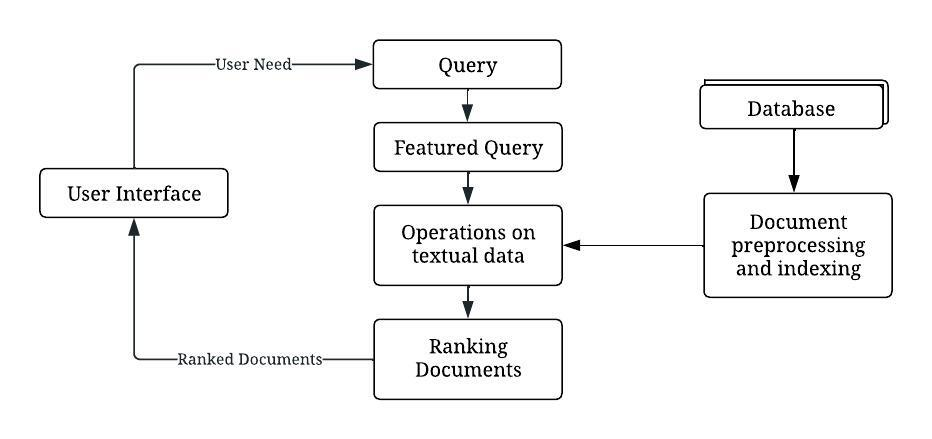
\includegraphics[width=\textwidth]{2Background/Background/IR.jpeg}
    \caption{Flowchart illustrating the information retrieval system process.}
    \label{fig:pipelines}
\end{figure}

Large Language Models (LLMs), often called state-of-the-art language models in Natural Language Processing (NLP), represent a remarkable advancement in machine learning technology. These models are designed to handle vast amounts of text data, allowing them to generate natural language text, answer questions, or make predictions. LLMs like GPT-3 and BERT have gained significant attention for their ability to comprehend and generate human-like text \cite{penha2022}.

LLMs find applications across a wide array of real-world scenarios. They power chatbots, which can engage in human-like conversations, making them invaluable for customer support and virtual assistants. They are integral in language translation services, breaking down language barriers and enabling seamless communication between individuals who speak different languages. Moreover, LLMs are the foundation for voice assistants, such as Siri or Alexa, enhancing their natural language understanding and response capabilities \cite{gpt}.

In addition to these applications, LLMs have unlocked new possibilities in content generation, language modelling, and text summarisation. They can craft coherent articles, stories, or reports, and they can serve as a foundation for more advanced language models. They can also distil lengthy documents into concise summaries, immensely valuable for tasks like content curation and automated news aggregation. Their versatility in understanding and generating text has made them a cornerstone of modern NLP research and applications.

Now, turning our attention to the domain of Information Retrieval (IR), retrieval pipelines play a pivotal role in efficiently searching and retrieving relevant information from extensive data collections, be it a document database or a search engine index. These pipelines encompass a series of well-defined processing steps to streamline the retrieval process:

\begin{itemize}
    \item Query Processing: This initial step involves processing user queries. During query processing, the system identifies relevant terms, expands the query with synonyms, and applies other query optimisation techniques to enhance the accuracy of the retrieval process.
    \item Document Indexing: In this step, the documents contained within the collection are indexed. Document indexing involves the transformation of documents into a more manageable format, often through token embedding techniques. This transformed data structure facilitates faster and more efficient searching.
    \item Ranking: Following document indexing, documents are ranked based on their relevance to the user's query. Various models and algorithms are applied to assign scores to documents, allowing for the sorting of documents by their perceived relevance.
    \item Presentation: The final stage of the retrieval pipeline involves presenting the search results to the user in a user-friendly format. This could be a list of documents with summaries, snippets, or other relevant metadata, making it easier for users to find and access the information they seek \cite{chen, zendel}.
\end{itemize}

It's important to note that retrieval pipelines can be further customised to cater to specific needs. Additional steps might include filtering or classifying search results based on domain-specific criteria or leveraging machine learning techniques to improve relevance comparisons. These advanced steps are particularly relevant in scenarios where precise and contextually relevant results are essential, such as in medical information retrieval \cite{lu}.